% generated by compose_fig8_schematic.sh; do not edit by hand
\documentclass[border=0pt]{standalone}
\usepackage[T1]{fontenc}
\usepackage{textcomp}
\usepackage{helvet}
\renewcommand{\familydefault}{\sfdefault}
\usepackage{sfmath}
\newcommand{\mi}{\mathbin{\text{\textminus}}}
\newcommand{\mneg}{\text{\textminus}}
\usepackage{amsmath}
\usepackage{graphicx}
\usepackage{tikz}
\definecolor{boxfill}{RGB}{237,238,250}
\begin{document}
\begin{tikzpicture}[x=1bp, y=1bp, inner sep=0pt, outer sep=0pt]
\node[anchor=south west] at (0,0) {\includegraphics{/home/yuzhengz/Manuscripts/My-Papers/Bayesian-ARGOS-Manuscript-CPR/schematic-plots/pyargos_with_sindy_shred.pdf}};
\node[anchor=south west] at (557.202,278.356) {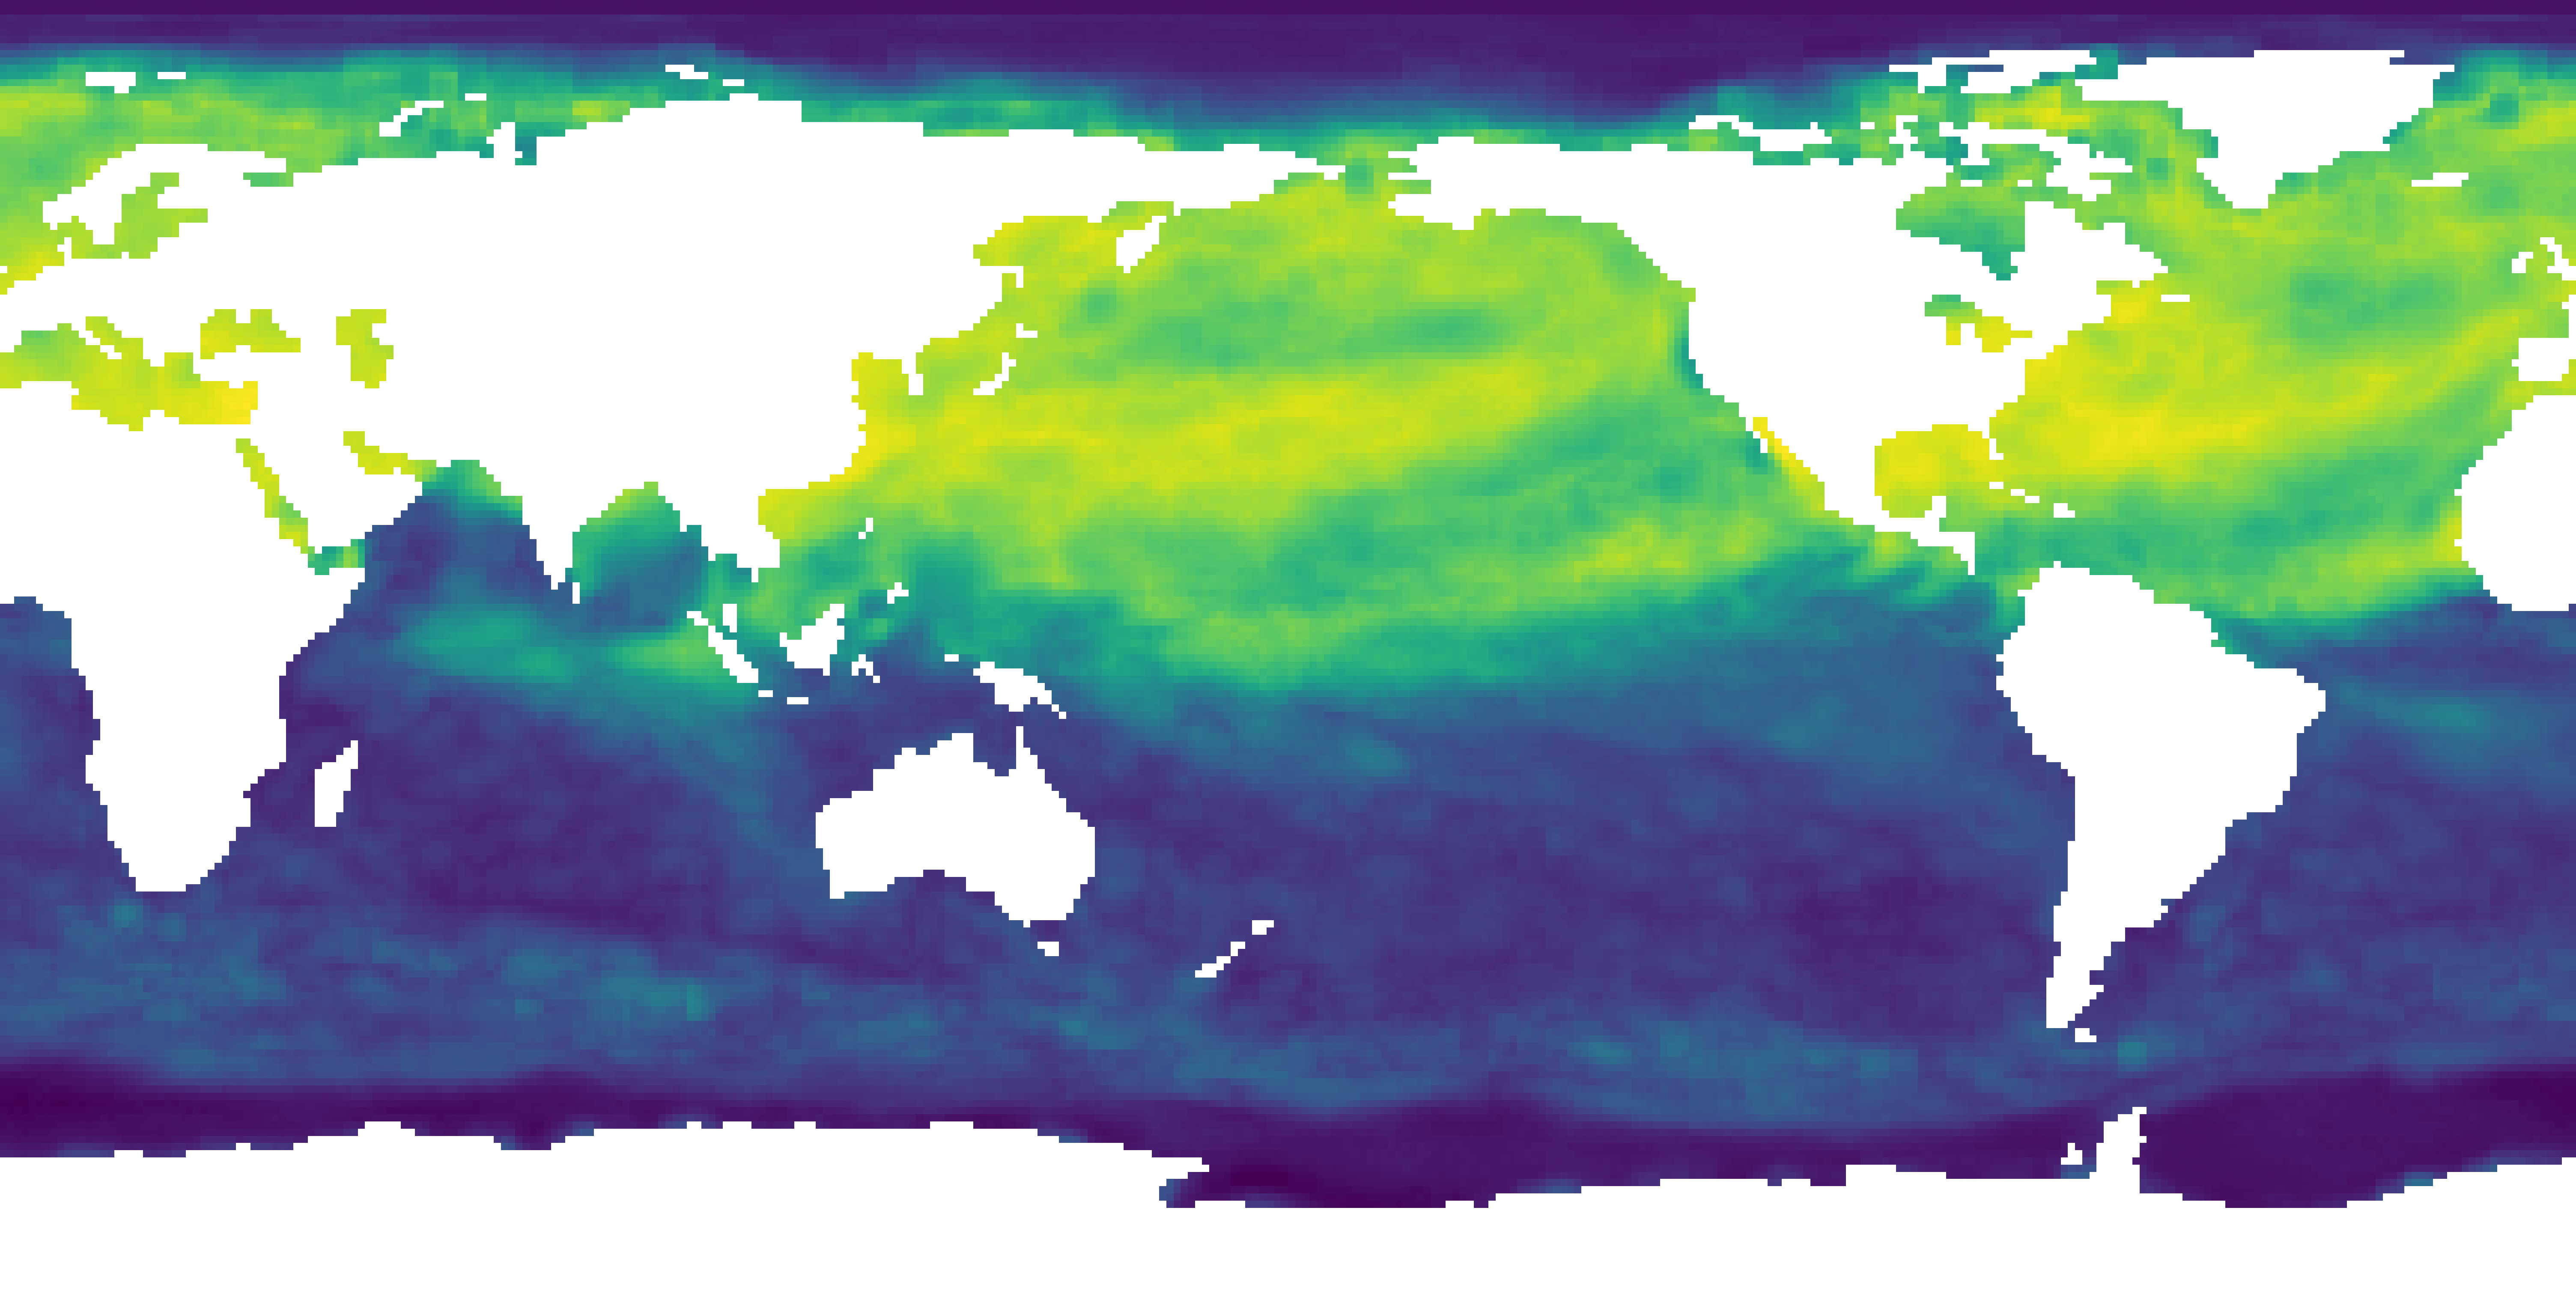
\includegraphics[width=293.195bp, height=147.204bp]{fig8_map_viridis.png}};
\node[anchor=south west] at (856.636,278.404) {
\includegraphics[width=7.359bp, height=147.155bp]{fig8_cbar_viridis.png}};
\fill[boxfill] (652,70) rectangle (894,161);
\begin{scope}[every node/.style={anchor=base west, font=\fontsize{14}{34}\selectfont}]
\node at (654.5,146.5) {$\dot{z}_1 = \mneg 0.98 + 8.16\,z_2 \mi 4.20\,z_3$};
\node at (654.5,113.4) {$\dot{z}_2 = 0.55 \mi 3.41\,z_2 + 6.15\,z_3$};
\node at (654.5,77.9)  {$\dot{z}_3 = 0.95 \mi 8.19\,z_2 + 3.43\,z_3$};
\end{scope}
\end{tikzpicture}
\end{document}
